\documentclass[a4j,twocolumn,uplatex]{jsarticle}
%\documentclass[a4j,twocolumn,uplatex]{jsarticle}

\usepackage[dvipdfmx]{graphicx}
\usepackage[dvipdfmx]{hyperref}
%\usepackage{pxjahyper}
\usepackage{url}
\setlength{\textheight}{275mm}
\headheight 5mm
\topmargin -30mm
\textwidth 185mm
\oddsidemargin -15mm
\evensidemargin -15mm
\pagestyle{empty}

\begin{document}
\title{TDD(テスト駆動開発)の意義}
\author{情報科学科 西谷研究室 2549 浦田 航貴}
\date{}
\maketitle
\section{TDD(Test Driven Development)とは}

2000年代初期に開発手法として確立された「テスト駆動開発」(Test Driven Development)は,その後10年もの間で普及が進み,今や珍しくない開発スタイルの1つとなっている.国内でも「アジャイルアカデミー」「TDD Boot Camp」などによる推進・普及活動が各地で活発化し,認知が広がっている\cite{1}.

テスト駆動開発は,テストファーストによる追加・変更と、リファクタリングによる設計改善という,2つの活動で構成されます.継続的にユニットテストを使って設計検討やチェック,リファクタリングを行うことにより,テスタビリティに優れバグの少ないソースコードを実現することができます.またTDDの運用に当たっては,プログラミングの中で軽快かつスムーズに利用できるユニットテスティングフレームワークが重要です\cite{1}.

\section{テスティングフレームワークについて}
Rubyは標準ライブラリとして,minitest/unitというテスティングフレームワークを提供している.このライブラリはユーザレベルでの互換性がある.Test::Unit APIはRubyの標準配布物に一部であり,ハックしたり拡張するのが基本的に簡単でである.既存のテスティングフレームワークの多くはTest::Unitをもとにして作られており,Ruby開発者としてTest::Unitについて実践的な知識を持ち合わせておく必要がある.

\section{テスト駆動開発の流れ}
\begin{center}
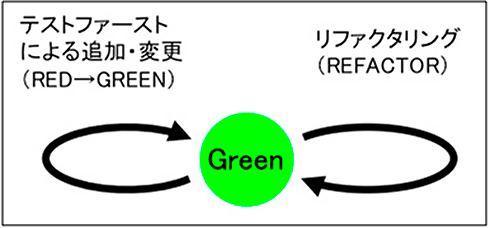
\includegraphics[width=6cm]{TDD.png}
\\{図1: TDDの進め方.}
\end{center}


テスト駆動開発は以下のRED, GREEN, REFACTORという3つの作業サイクルを細かく繰り返してプログラミングを進めていきます.

(1), RED  (失敗するテストを書く.)


(2), GREEN  (テストを成功させる最低限のコードを書く.)


(3), REFACTOR  (コードをリファクタリングして綺麗にする.)

リファクタリングは,コンピュータプログラミングにおいて,プログラムの外部から見た動作を変えずにソースコードの内部構造を整理することです.RED,GREENという言葉は,JUnitなどTDDで多用されるテスティングフレームワークの多くがテスト失敗を赤色表示で,テスト成功を緑色表示で通知することに由来している.このサイクルでは以下の2つの活動を実現します\cite{1}.


\subsection{テストファーストによる追加・変更}


最初に失敗するテストを書き,次にそれを成功させる最低限のコードを書く,というステップを繰り返すことでプログラミングを進めていきます.このテストを書いてコードを書くまでのサイクルは,テスト駆動開発では超短期で実行します.


\subsection{リファクタリングによる設計改善}


テストファーストでプログラミングを進めるうちにソースコードが粗雑になってきたら,ソースコードをリファクタリングして綺麗にします.リファクタリングではテストファーストで作成したテストを回帰テストとして活用します.

\section{TDDの目的と効果}
TDDの主な目的としては,軽快なフィードバックの確保,きれいで動くコードの確保などによる,開発の改善が挙げられている. TDDの効果としては,例えば組織として展開した場合,実行工数を15%から25%増加させる代わりに,欠陥密度を4割から9割低下させてデバッグや手戻り工数を減少させ,トータルの総工数を削減するといった事例が報告されている\cite{1}.

またテストを書くことはコードをよりよくメンテナンス可能にするためにあると覚えておくことが重要である.混乱させるためではないし,実際のコーディングの代わりに時間のかかる作業で行き詰まりを感じさせるためではない.コードを書く前にテストを書き,小さな機能スパイクごとにコードをきれいにすることによって,複雑すぎるコードにありがちな落とし穴を簡単に回避できるようになる.\cite{2}.


\begin{flushleft}
\begin{thebibliography}{9}
\bibitem{1}「テスト駆動開発/振る舞い駆動開発を始めるための基礎知識」,井芹洋輝 \url{http://www.atmarkit.co.jp/ait/articles/1403/05/news035_3.html}.
\bibitem{2} 「Ruby ベストプラクティス」, Gregory Brown, 第1章
\end{thebibliography}
\end{flushleft}
\end{document}